\chapter{软件概述}
\section{启动}

如图 \ref{fig:启动} 所示，文件夹内有三个文件，即“优秀学生奖学金加分项目评审软件.exe”，“users.json”，“logo.ico”，其三者分别是软件本体程序，用户信息存储文件，软件图标。第一次访问启动软件后，才会生成“users.json”。

用户可通过双击或鼠标右键展开菜单的方式打开（启用）“优秀学生奖学金加分项目评审软件.exe”，即实现启动软件。
\begin{figure}[h]
	\centering
	\small
	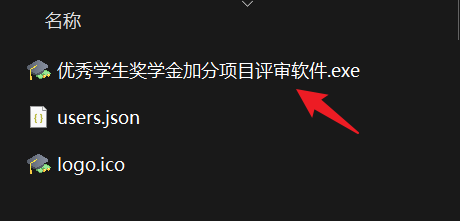
\includegraphics[width=0.3\linewidth]{fig/启动}
	\caption{软件的启动}
	\label{fig:启动}
\end{figure}


正常启动软件后，界面如图\ref{fig:启动界面}所示。
\begin{figure}[H]
	\centering
	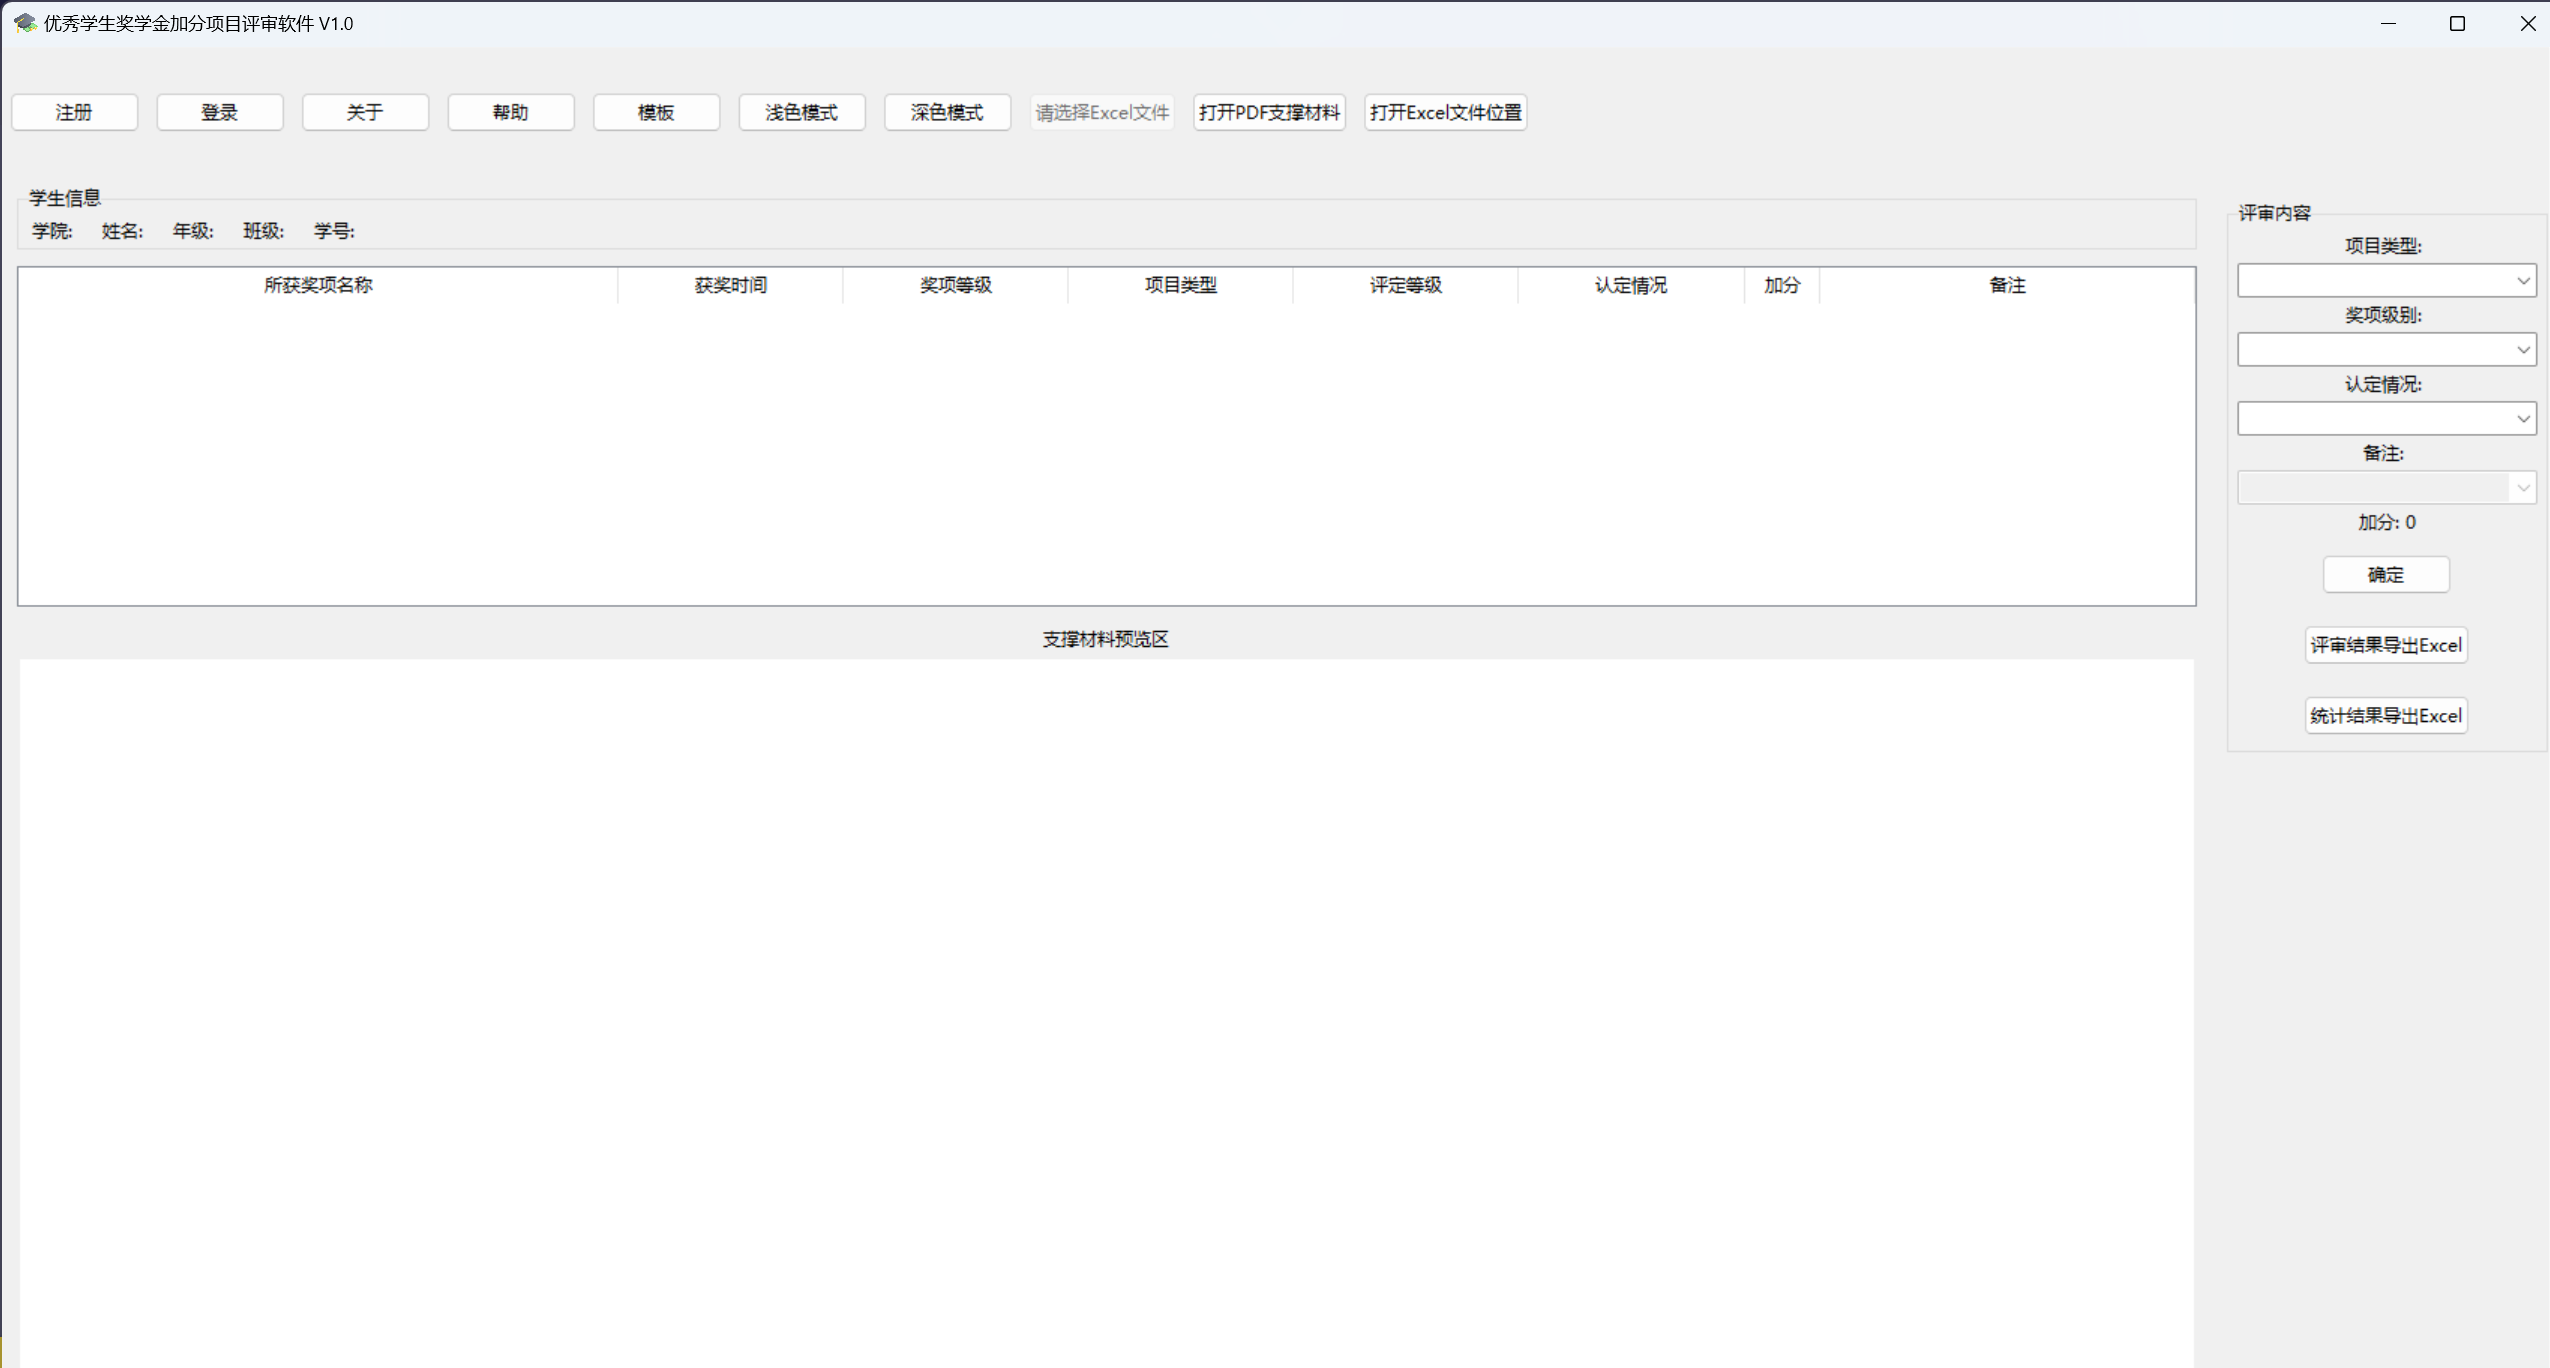
\includegraphics[width=0.5\linewidth]{fig/初始界面}
	\caption{版本V1.0的启动界面}
	\label{fig:启动界面}
\end{figure}


{\color{mygreen}	
	版本V2.0的启动界面如图\ref{fig:2.0启动界面}所示。
	\begin{figure}[H]
		\centering
		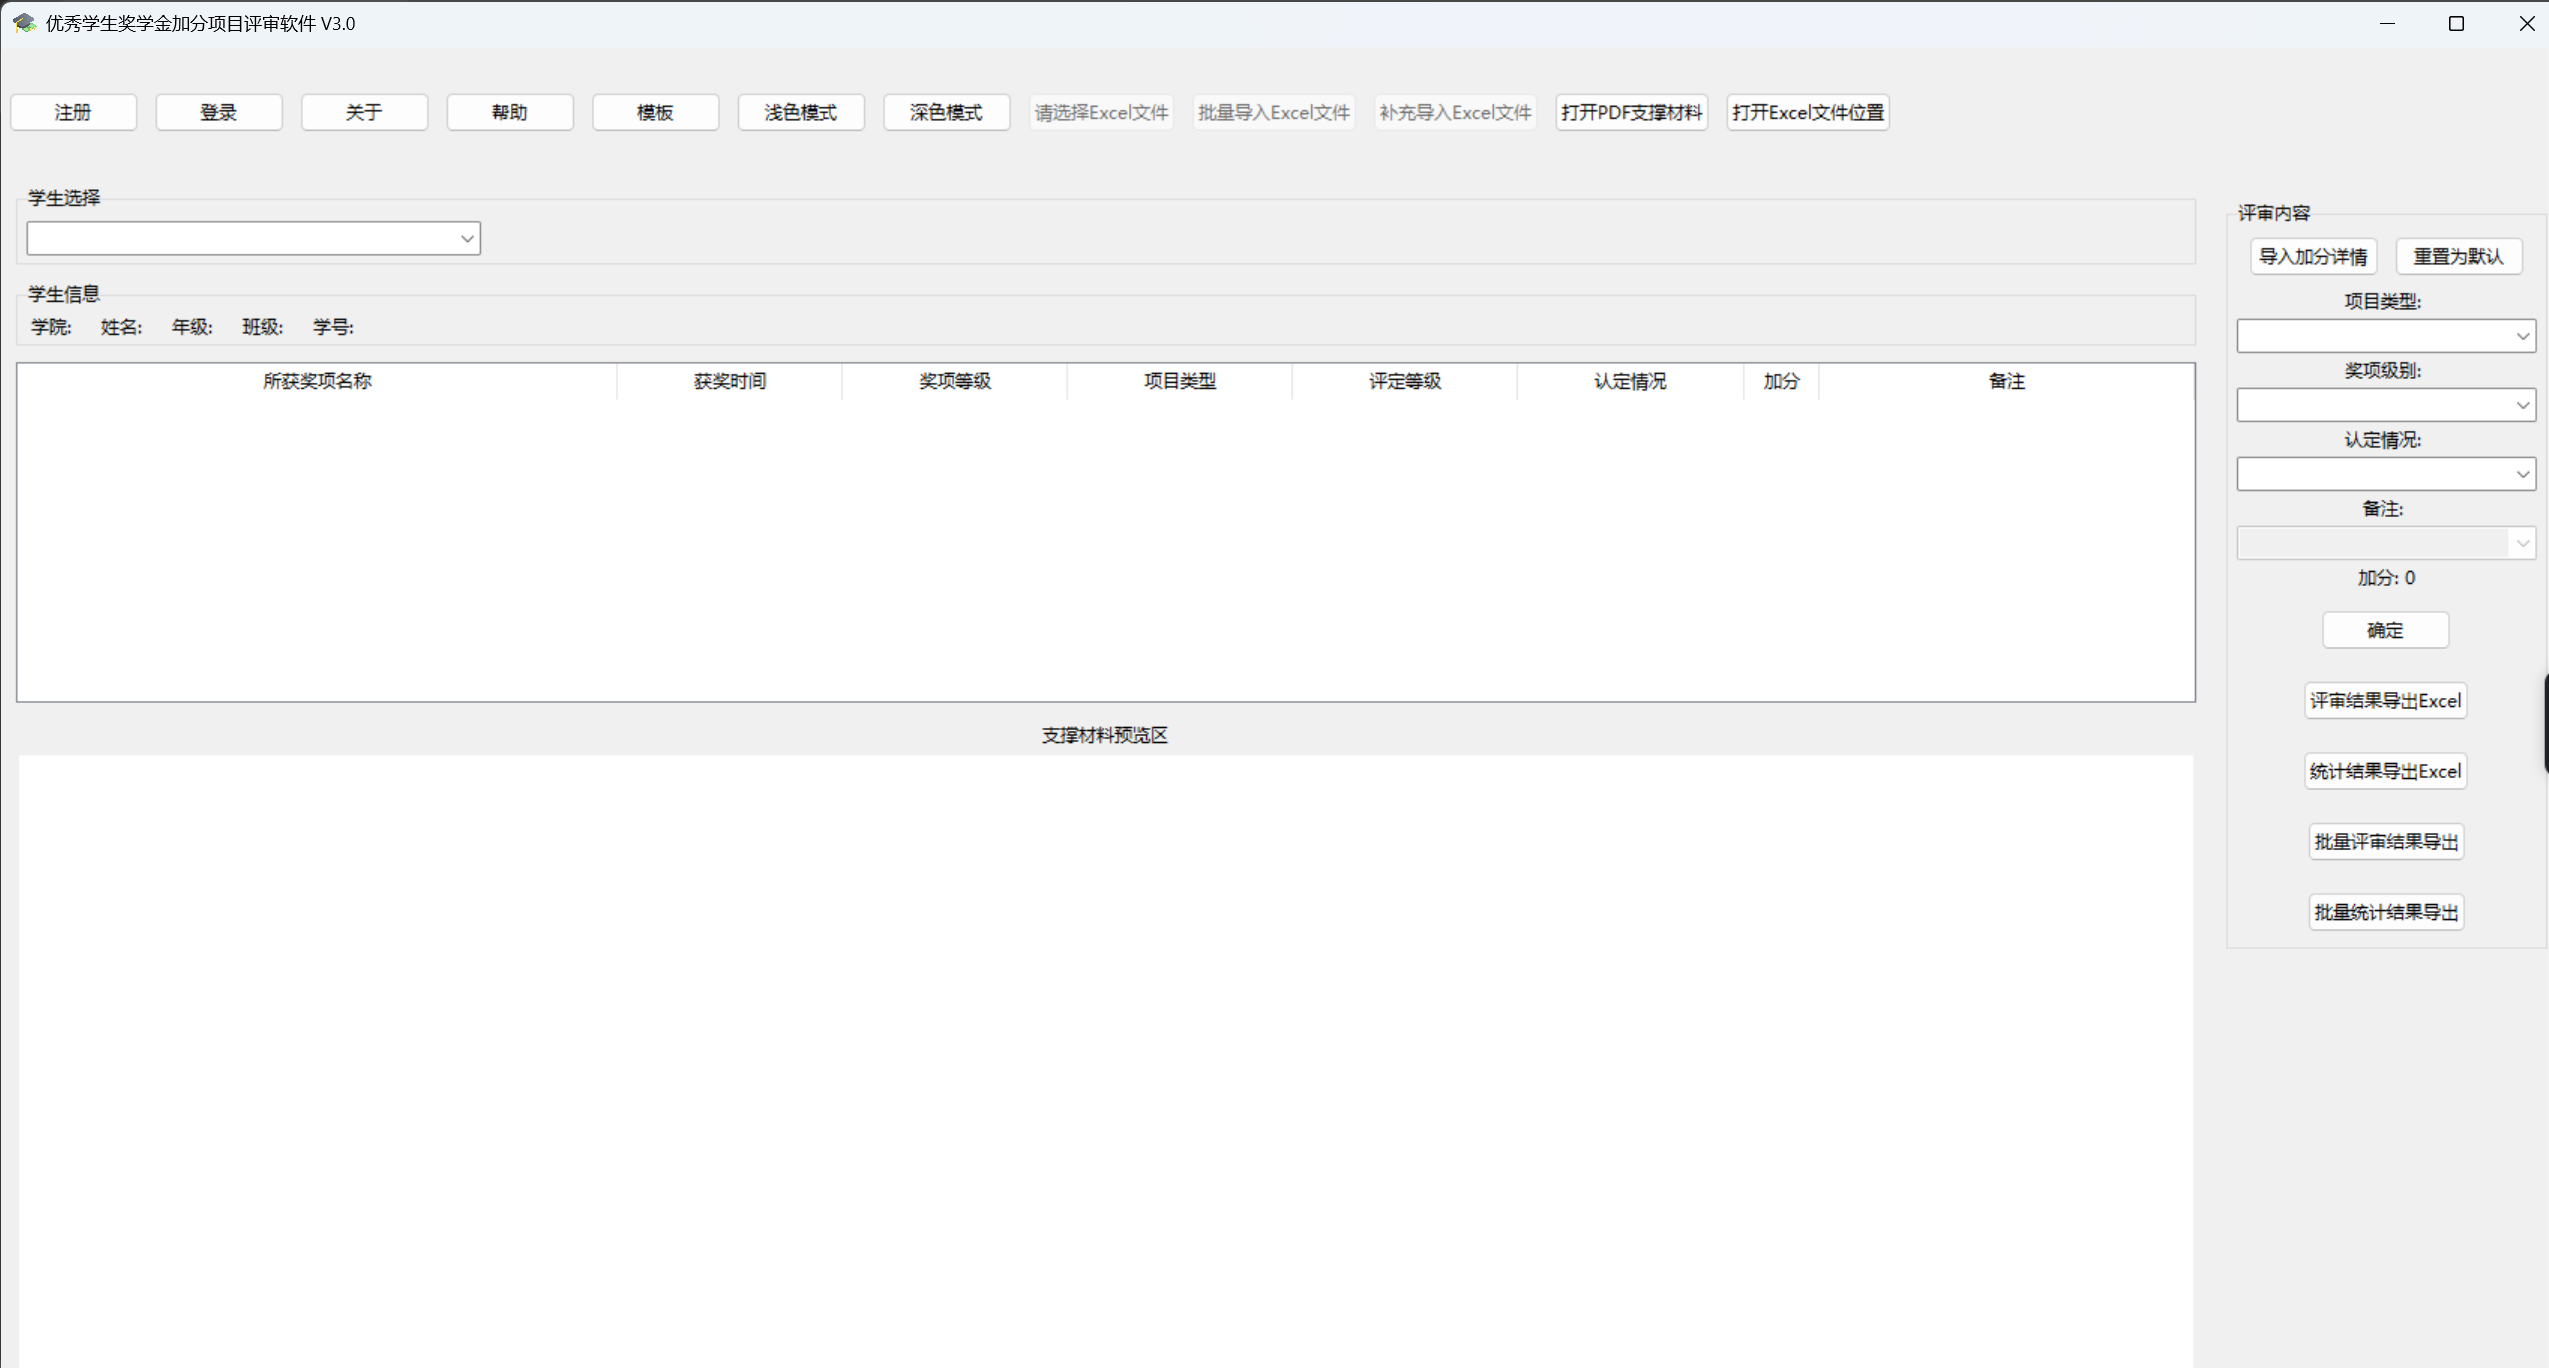
\includegraphics[width=0.5\linewidth]{fig/2.0初始界面}
		\caption{版本V2.0的启动界面}
		\label{fig:2.0启动界面}
	\end{figure}
}

	{\color{myred}
	版本V3.0新增了"数据库（可选）"能力：当用户需要对历史评审数据进行查询、导出或追溯操作日志时，可通过配置文件启用数据库功能。数据库默认使用 SQLite（Python 内置，无需安装额外数据库服务），数据自动存储在 \texttt{data/scholarship.db}；当不启用数据库时，软件原有功能不受影响。
}

	{\color{myred}
	其中新增/涉及的关键文件包括：\texttt{db\_config.json}（数据库连接配置，默认启用 SQLite，可由\texttt{db\_config.example.json}复制得到）、\texttt{database/}目录（数据库模块，包含连接管理、数据模型、业务服务等）。
}

\newpage
\section{界面介绍}
\subsection{导航栏}

如图\ref{fig:导航栏}所示，导航栏位于界面的左上角，共有7个操作按钮，分别是注册、登录、关于、帮助、模板、浅色模式、深色模式（默认启动为浅色模式）、文件导入按钮、打开PDF支撑材料、打开Excel文件位置。

\begin{figure}[H]
	\centering
	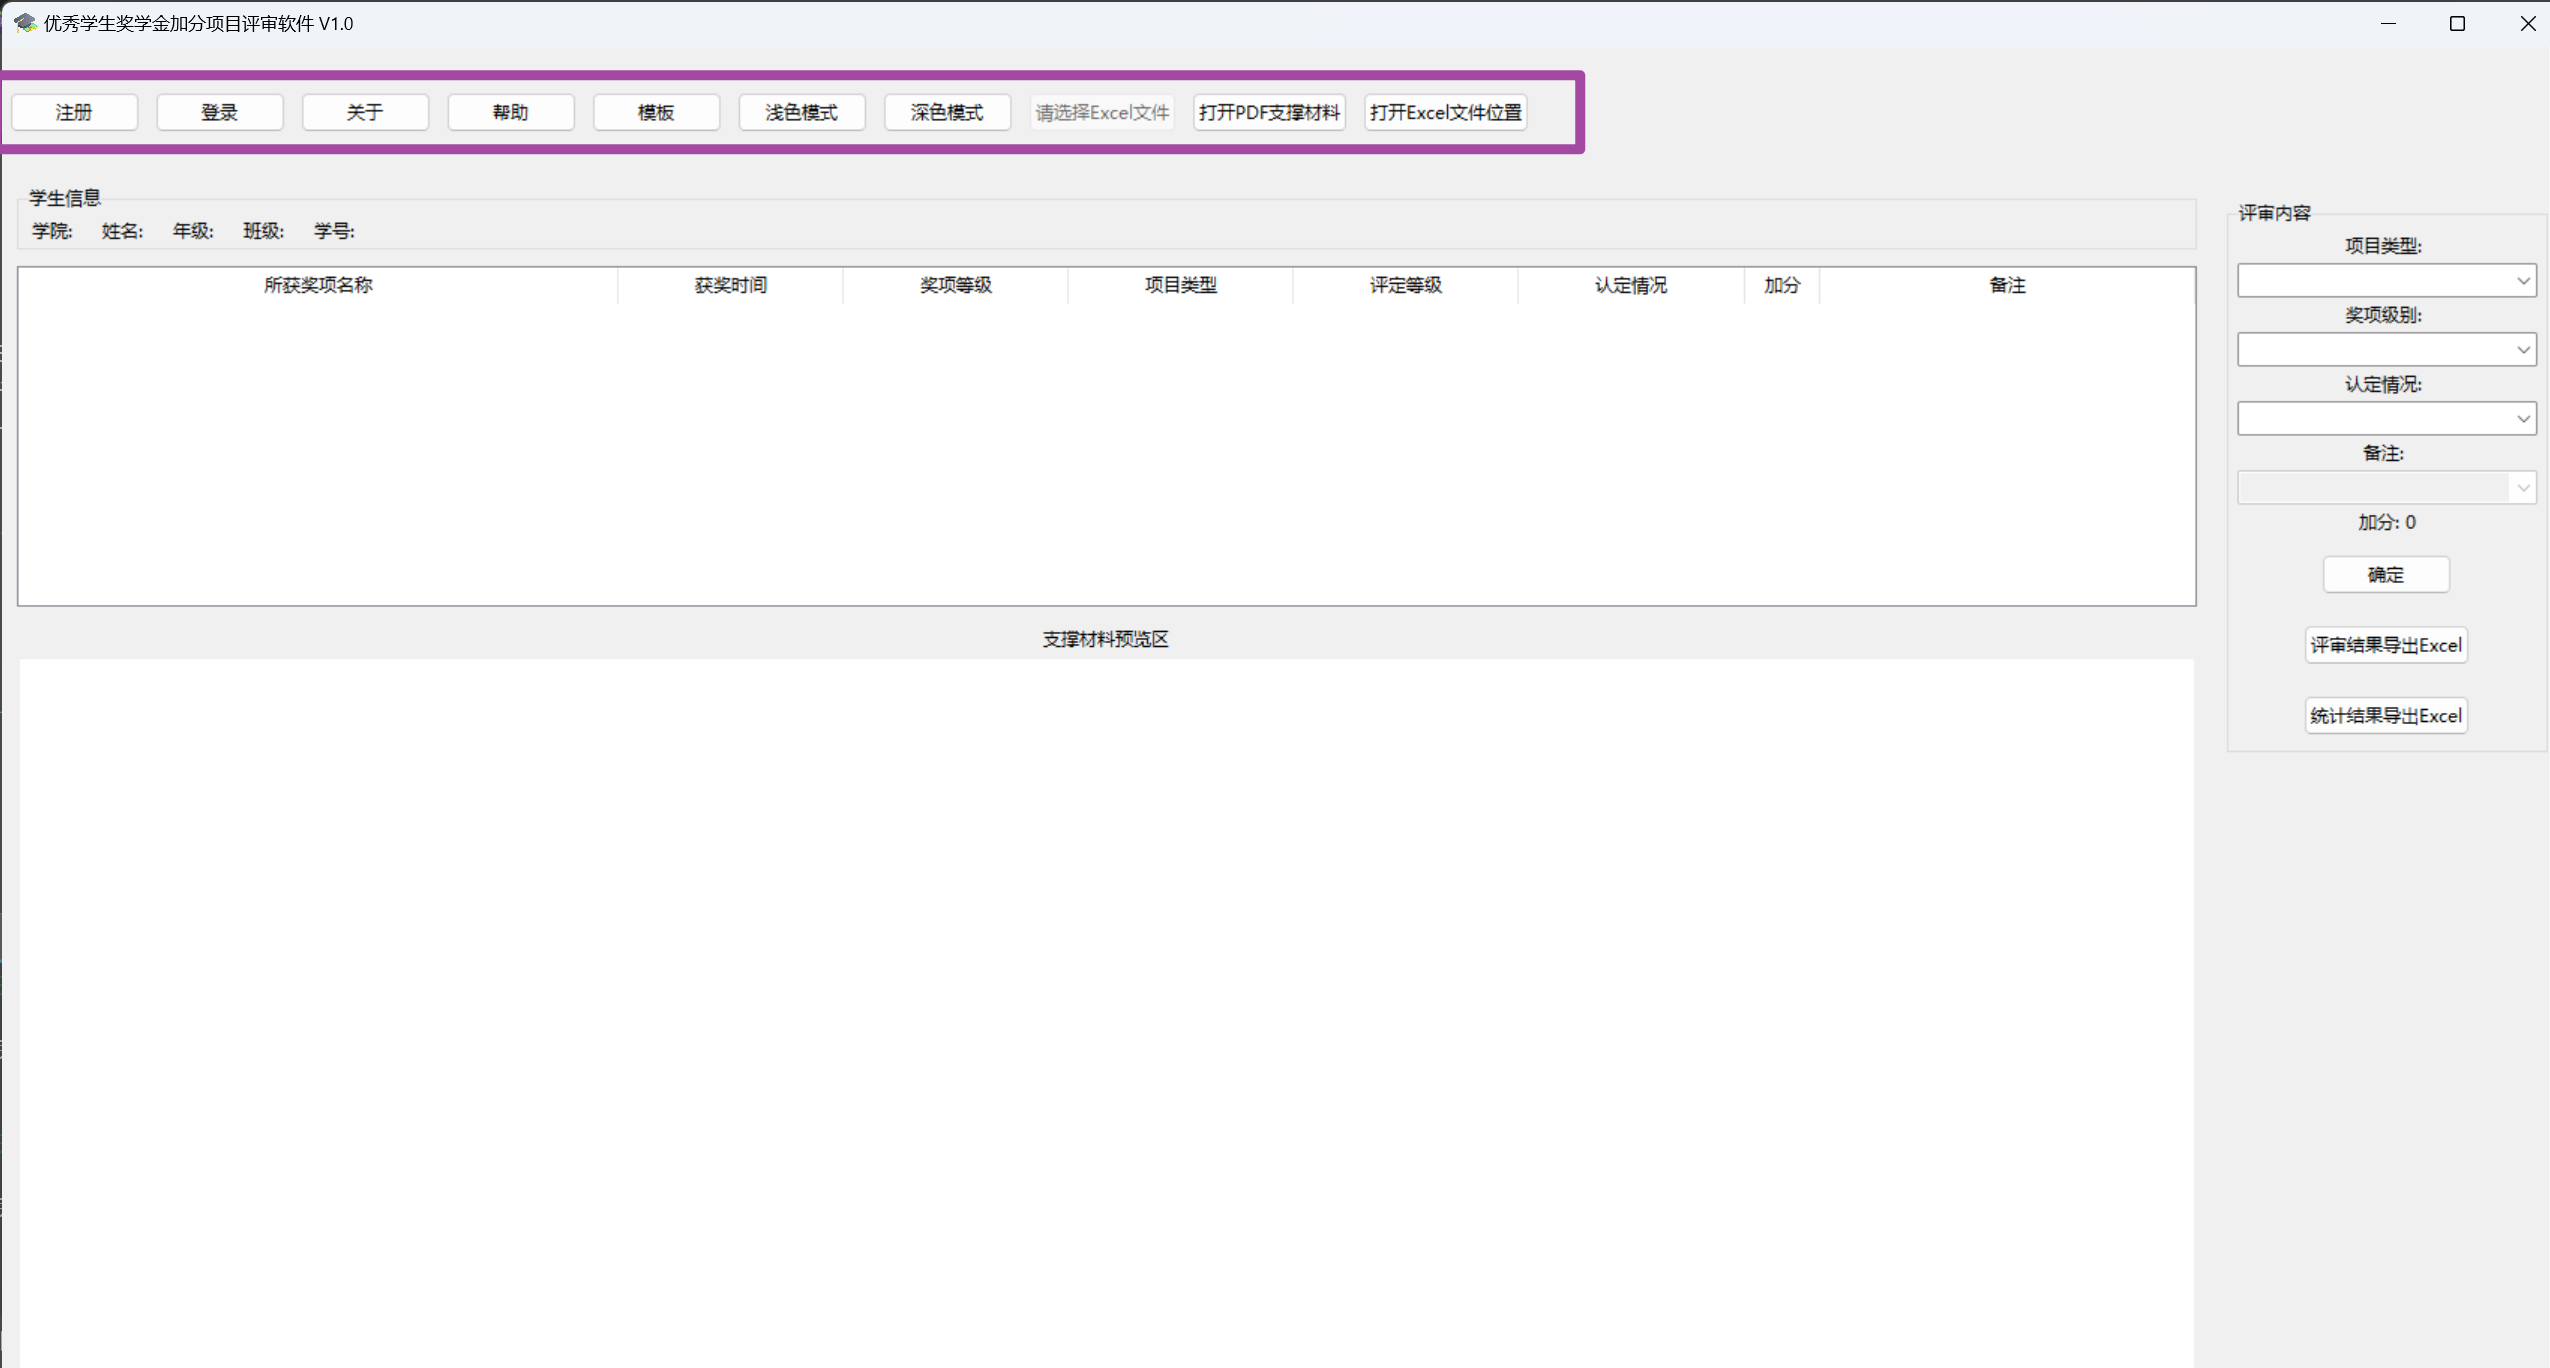
\includegraphics[width=0.7\linewidth]{fig/导航栏}
	\caption{导航栏}
	\label{fig:导航栏}
\end{figure}

{\color{mygreen}
	如图\ref{fig:2.0导航栏}所示，版本V2.0的导航栏新添加了“批量导入Excel文件”按钮和“补充导入Excel文件”按钮。
}
\begin{figure}[H]
	\centering
	
\includegraphics[width=1\linewidth]{fig/2.0导航条}
	\caption{版本V2.0的导航栏}
	\label{fig:2.0导航栏}
\end{figure}

{\color{myred}
	版本V3.0在导航栏新增了“管理”按钮。该按钮默认隐藏，仅当以管理员（admin）身份登录后才会在“登录”按钮左侧显示。点击“管理”按钮可打开管理员面板，进行用户解锁、角色切换、删除用户等管理操作。
	% 【需补充截图：V3.0导航栏——管理员登录后显示“管理”按钮的界面，命名为 fig/V3.0_navbar_admin.png】
}

\subsection{文件导入按钮}

如图\ref{fig:2.0文件导入}所示，文件导入按钮“请选择Excel文件”位于导航栏中，默认为暗色（不要可点选），只有登录后才可点选。
\begin{figure}[!ht]
	\centering
	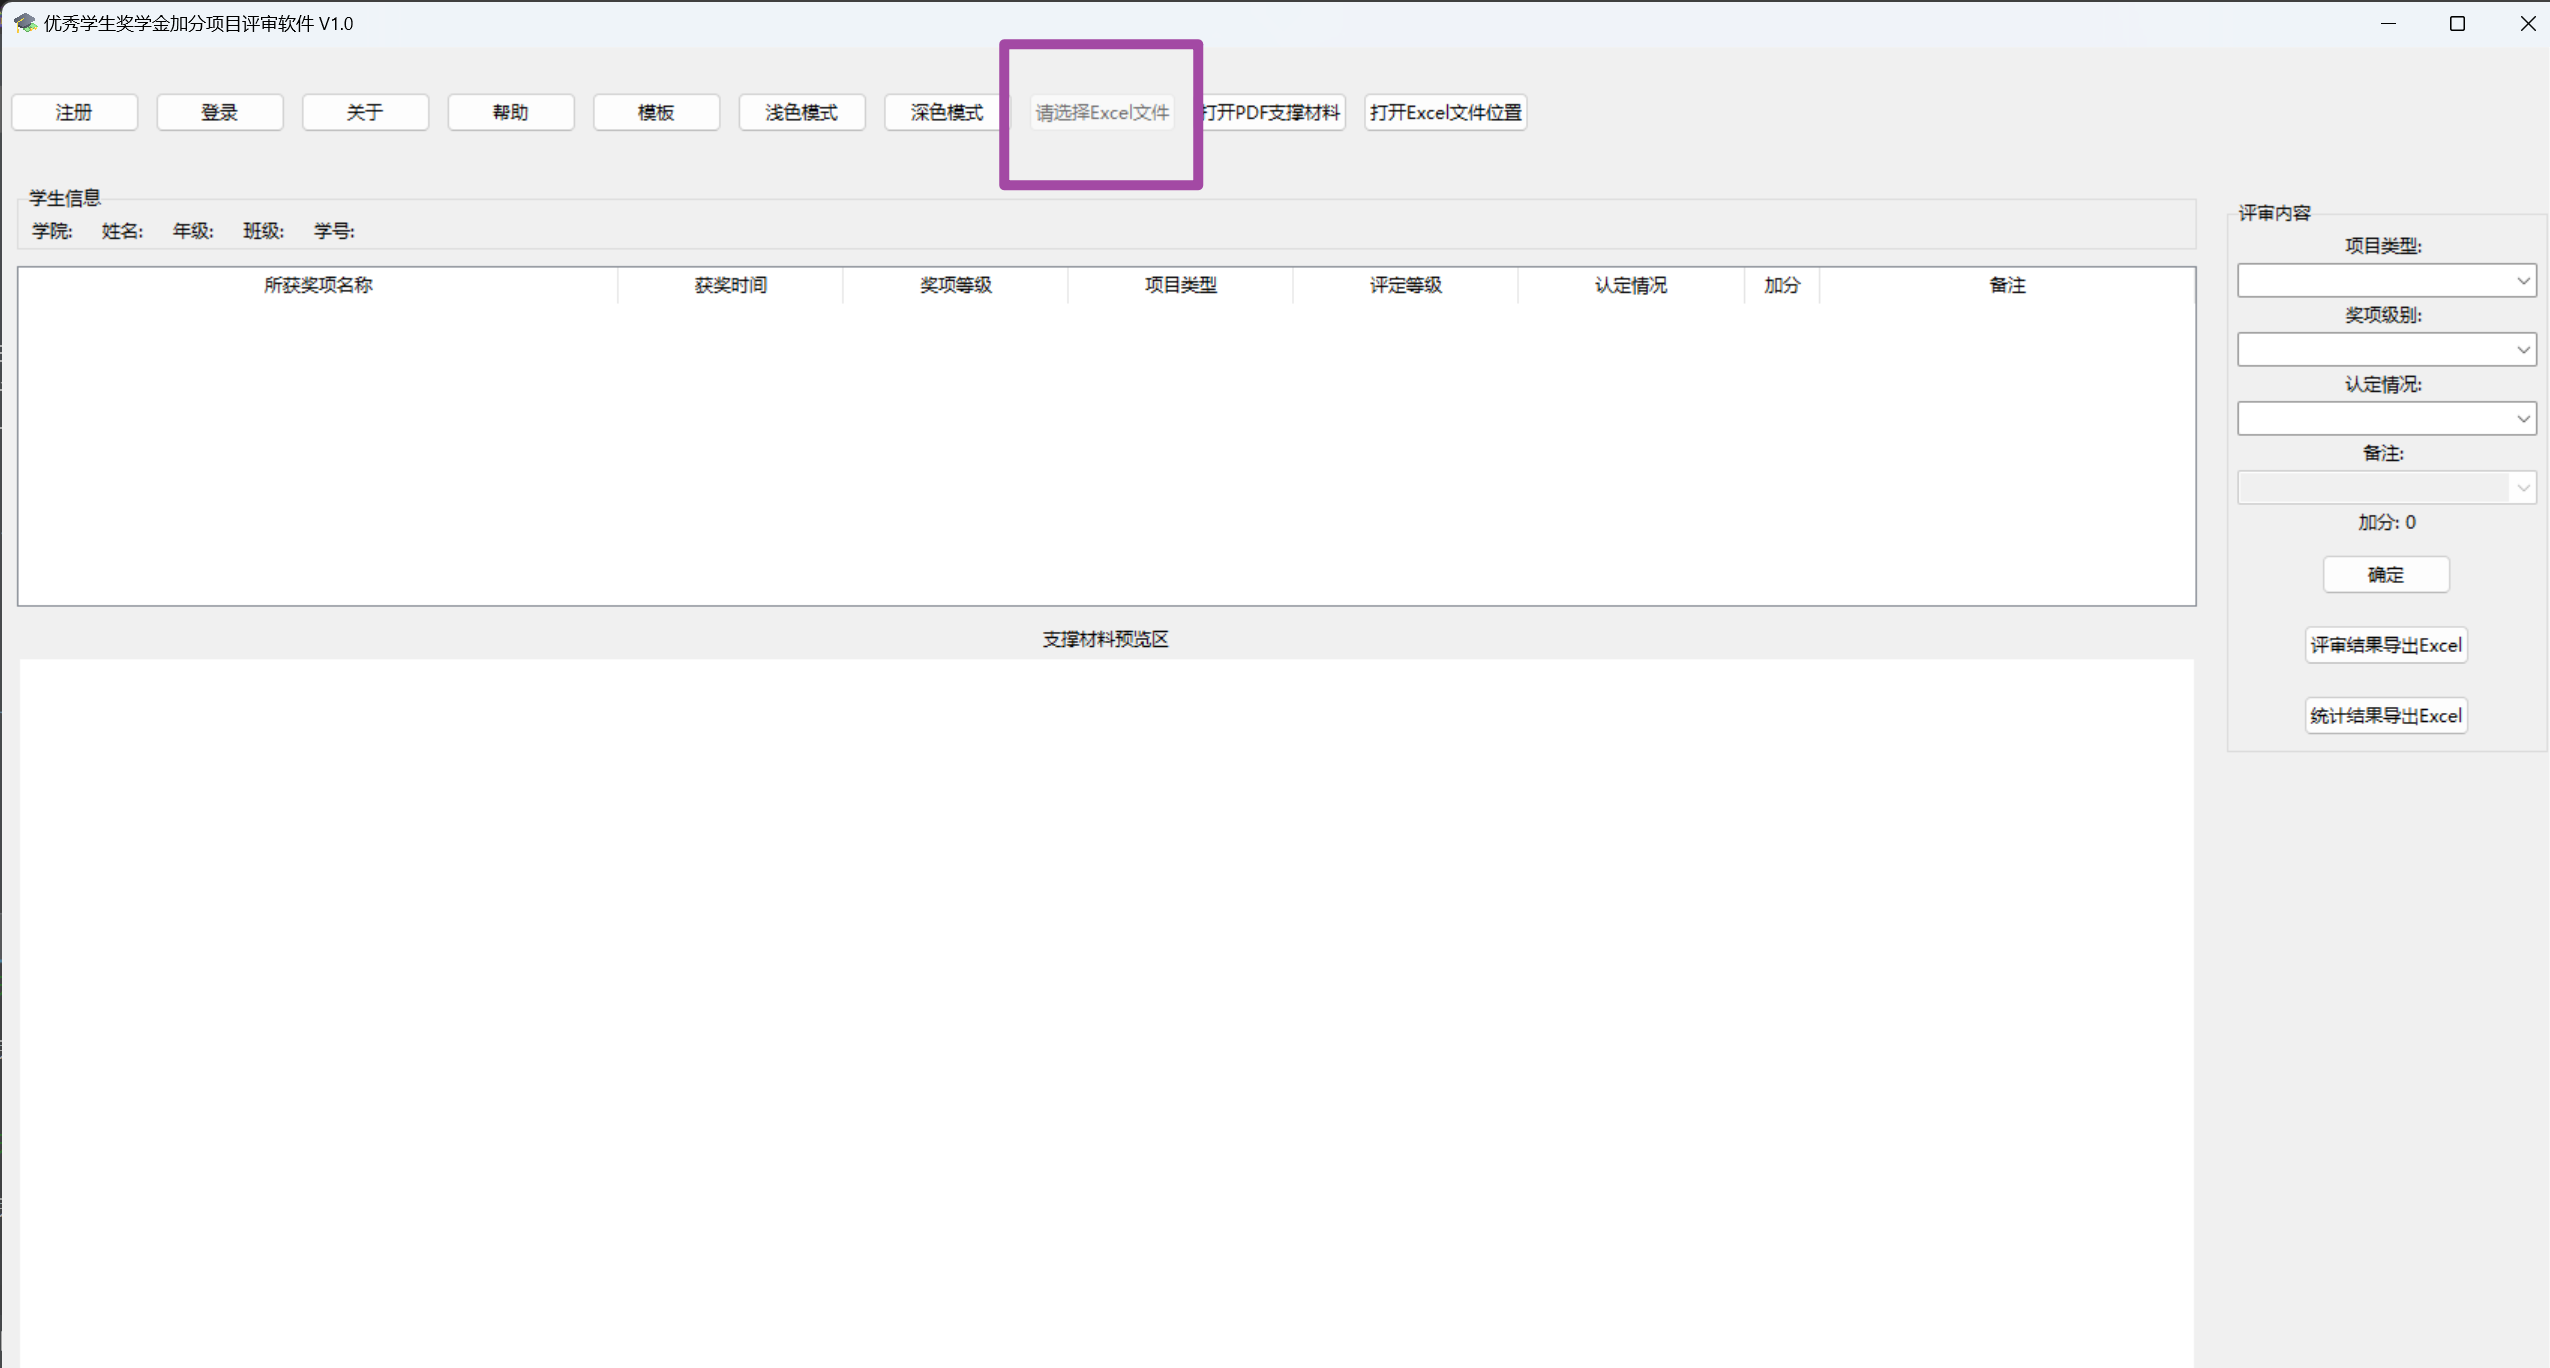
\includegraphics[width=0.7\linewidth]{fig/2.0文件导入}
	\caption{文件导入按钮}
	\label{fig:2.0文件导入}
\end{figure}


{\color{mygreen}
	如图\ref{fig:3.0文件导入}所示，版本V2.0支持“批量导入Excel文件”和“补充导入Excel文件”这两个文件导入功能，两个功能按钮默认为暗色（不要可点选），只有登录后才可点选。}
	\begin{figure}[!ht]
		\centering
		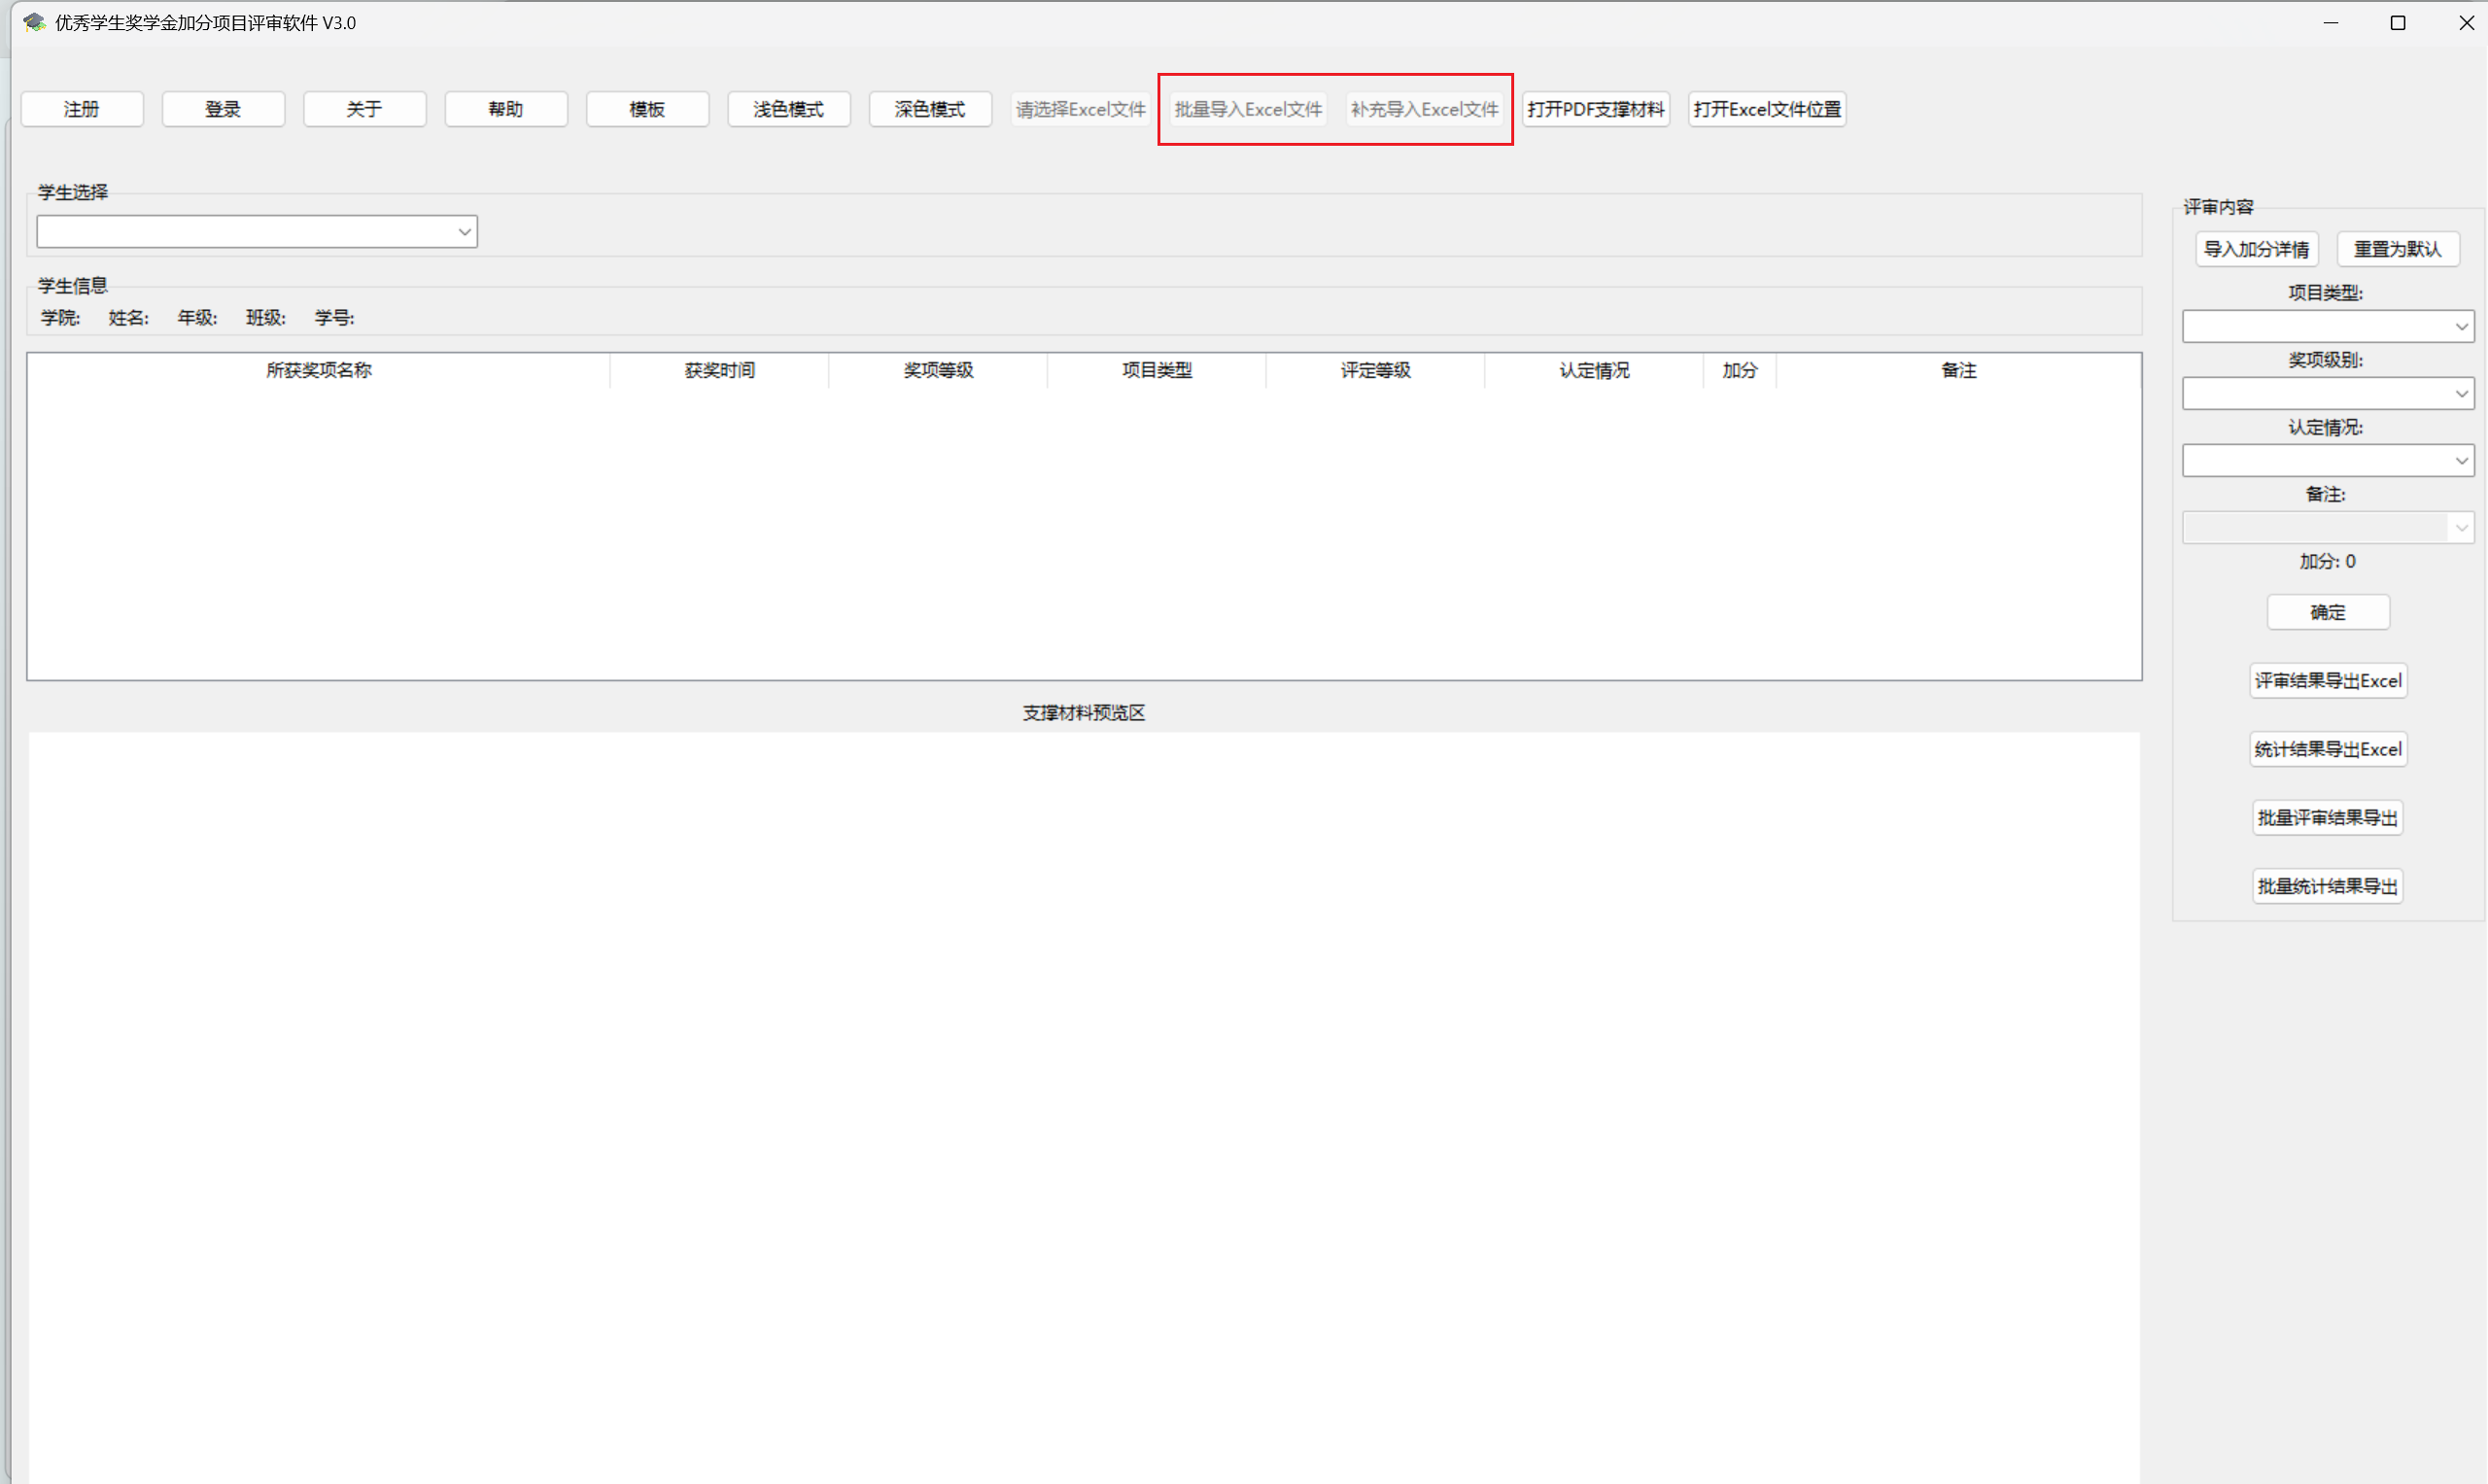
\includegraphics[width=0.7\linewidth]{fig/3.0文件导入}
		\caption{2.0文件导入按钮}
		\label{fig:3.0文件导入}
	\end{figure}
	



\subsection{评审界面}

如图\ref{fig:评审界面}所示，评审界面位于界面的中间位置，其分为三个片区，红框为读取导入文件后的学生信息，包括学院、姓名、年级、班级、学号；绿框为读取导入文件后的加分项目信息，包括所获奖项名称、获奖时间、奖项等级、项目类型、评定等级、认定情况、加分、备注；蓝框为读取评审人的评审操作按钮，包括对项目类型、奖项级别、认定情况、备注的下拉选择菜单，评审“确定”按钮，以及评审结果导出和统计结果导出两个按钮。
\begin{figure}[h]
	\centering
	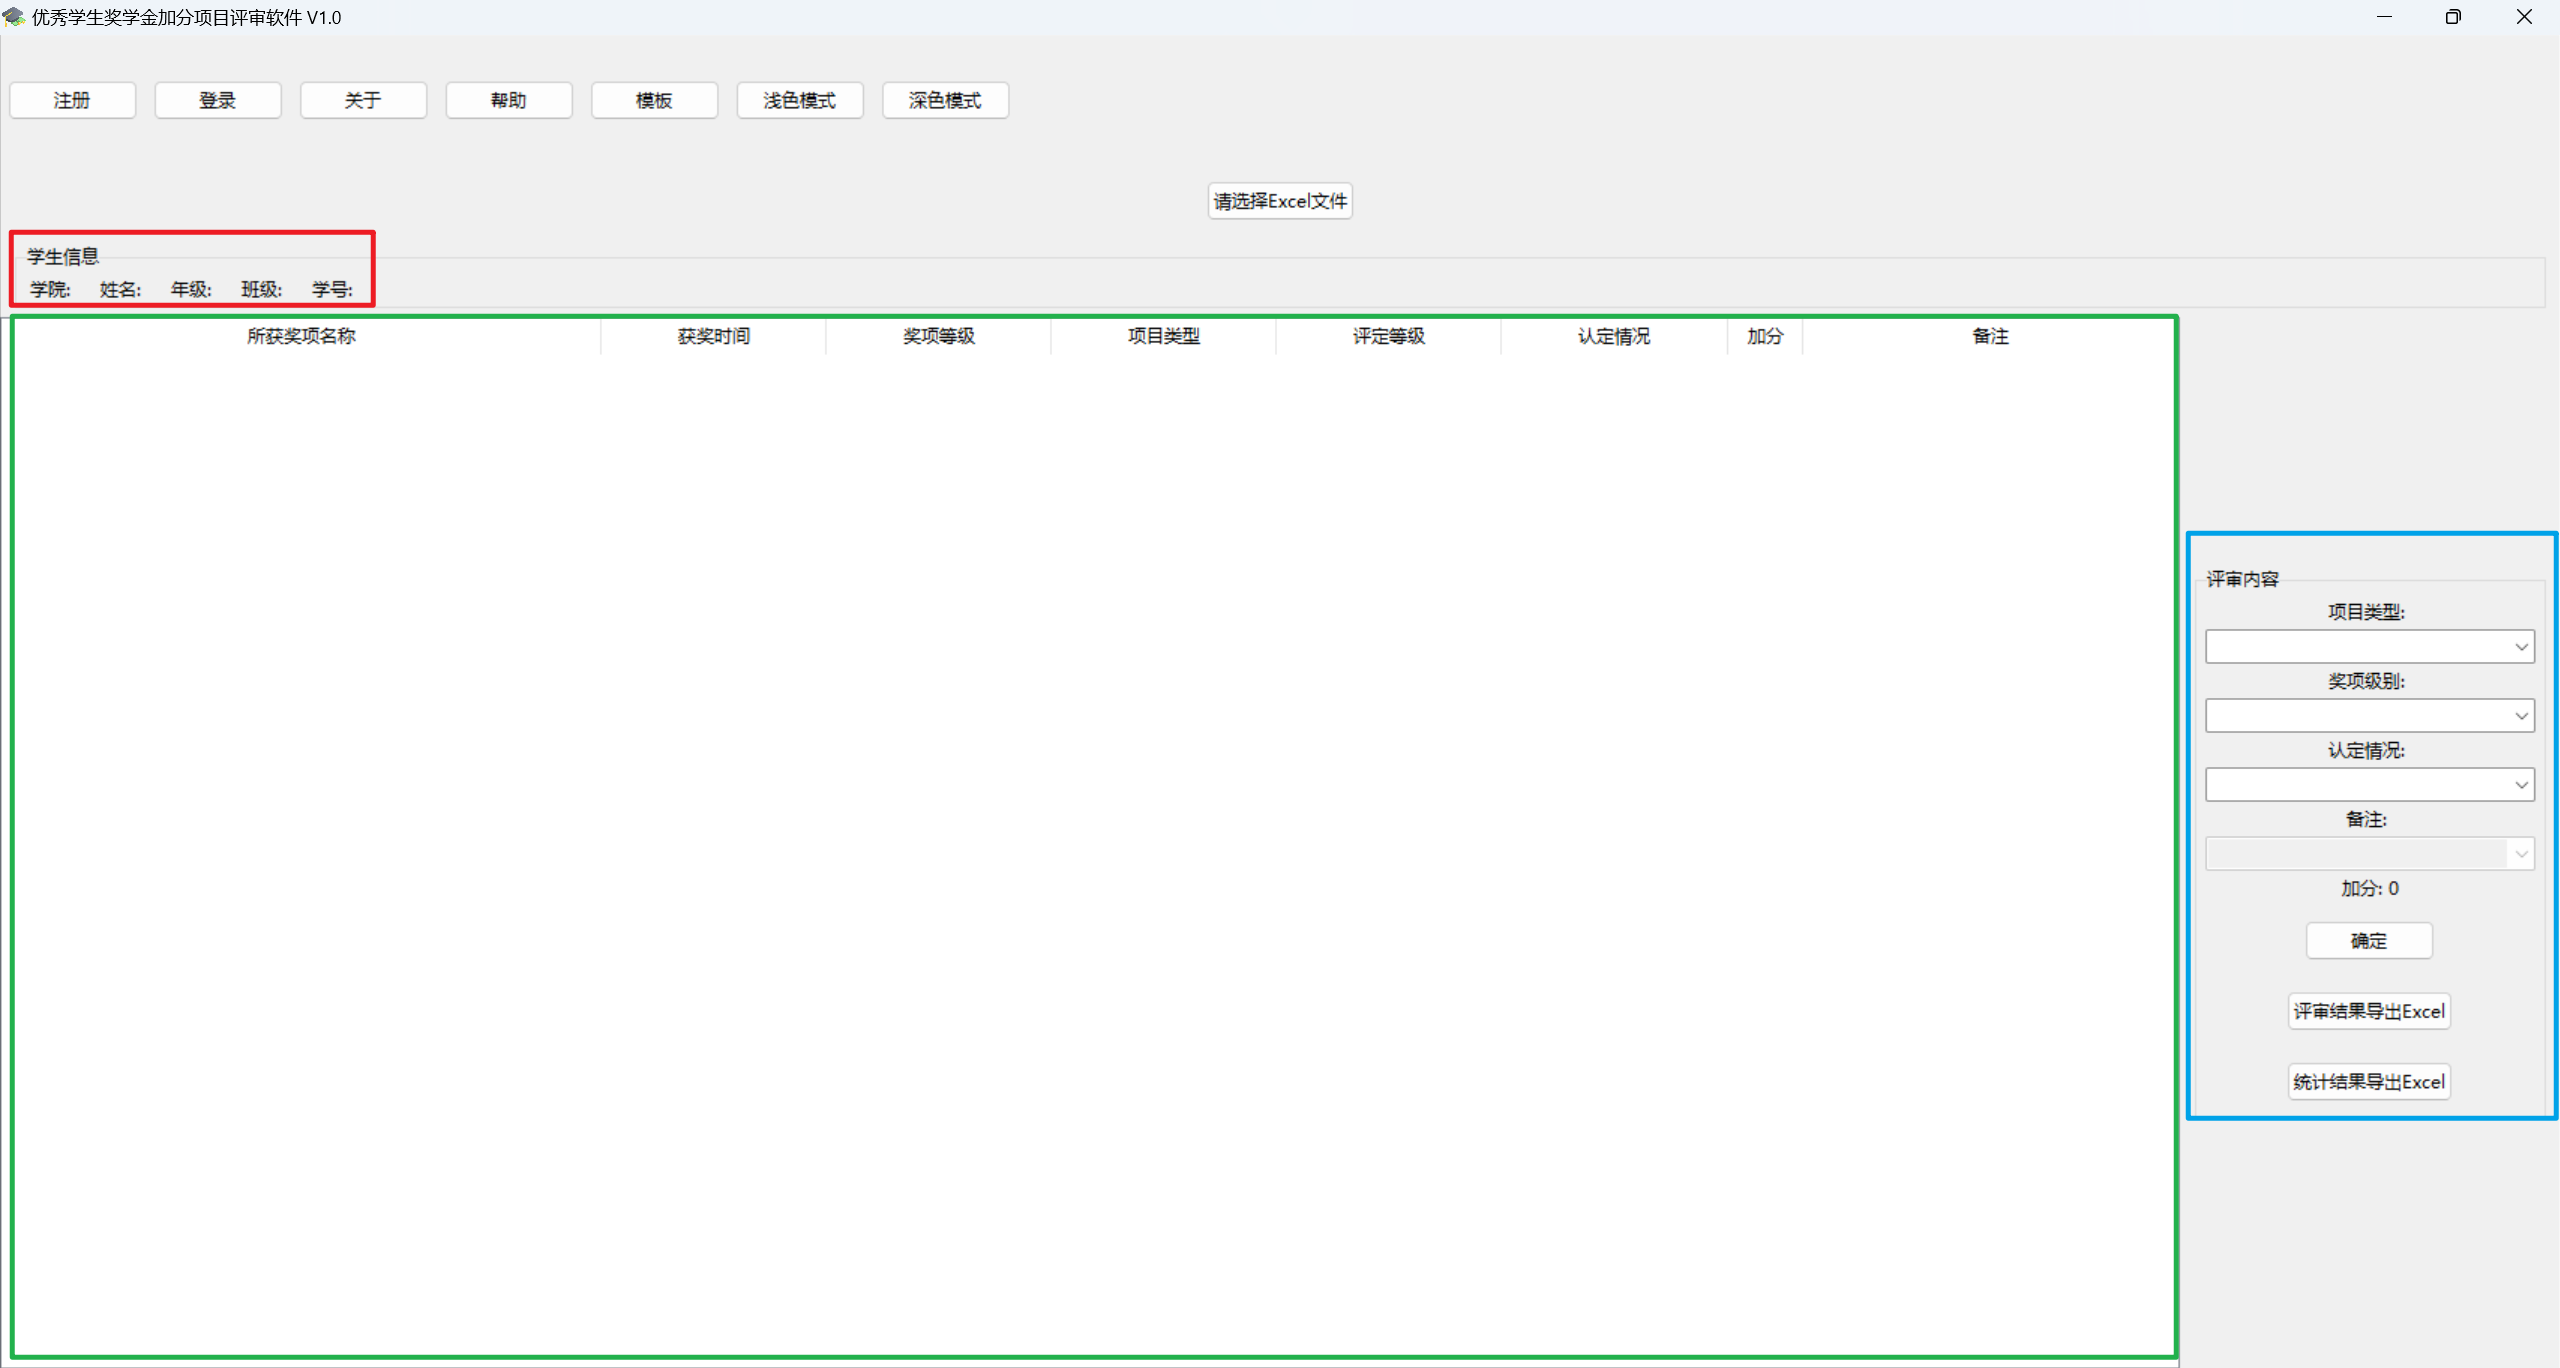
\includegraphics[width=0.7\linewidth]{fig/评审界面}
	\caption{评审界面}
	\label{fig:评审界面}
\end{figure}

{\color{mygreen}
	如图\ref{fig:版本V3.0评审界面新功能按钮展示}所示，为版本V2.0的评审界面，在学生信息的上方新增加了“学生选择”下拉菜单；在评审内容区域，新增加了“导入加分详情”按钮、“重置为默认”按钮、“批量评审结果导出”按钮、“批量统计结果导出”按钮，其各自功能将在后续章节内容进行阐述。
}
\begin{figure}[h]
	\centering
	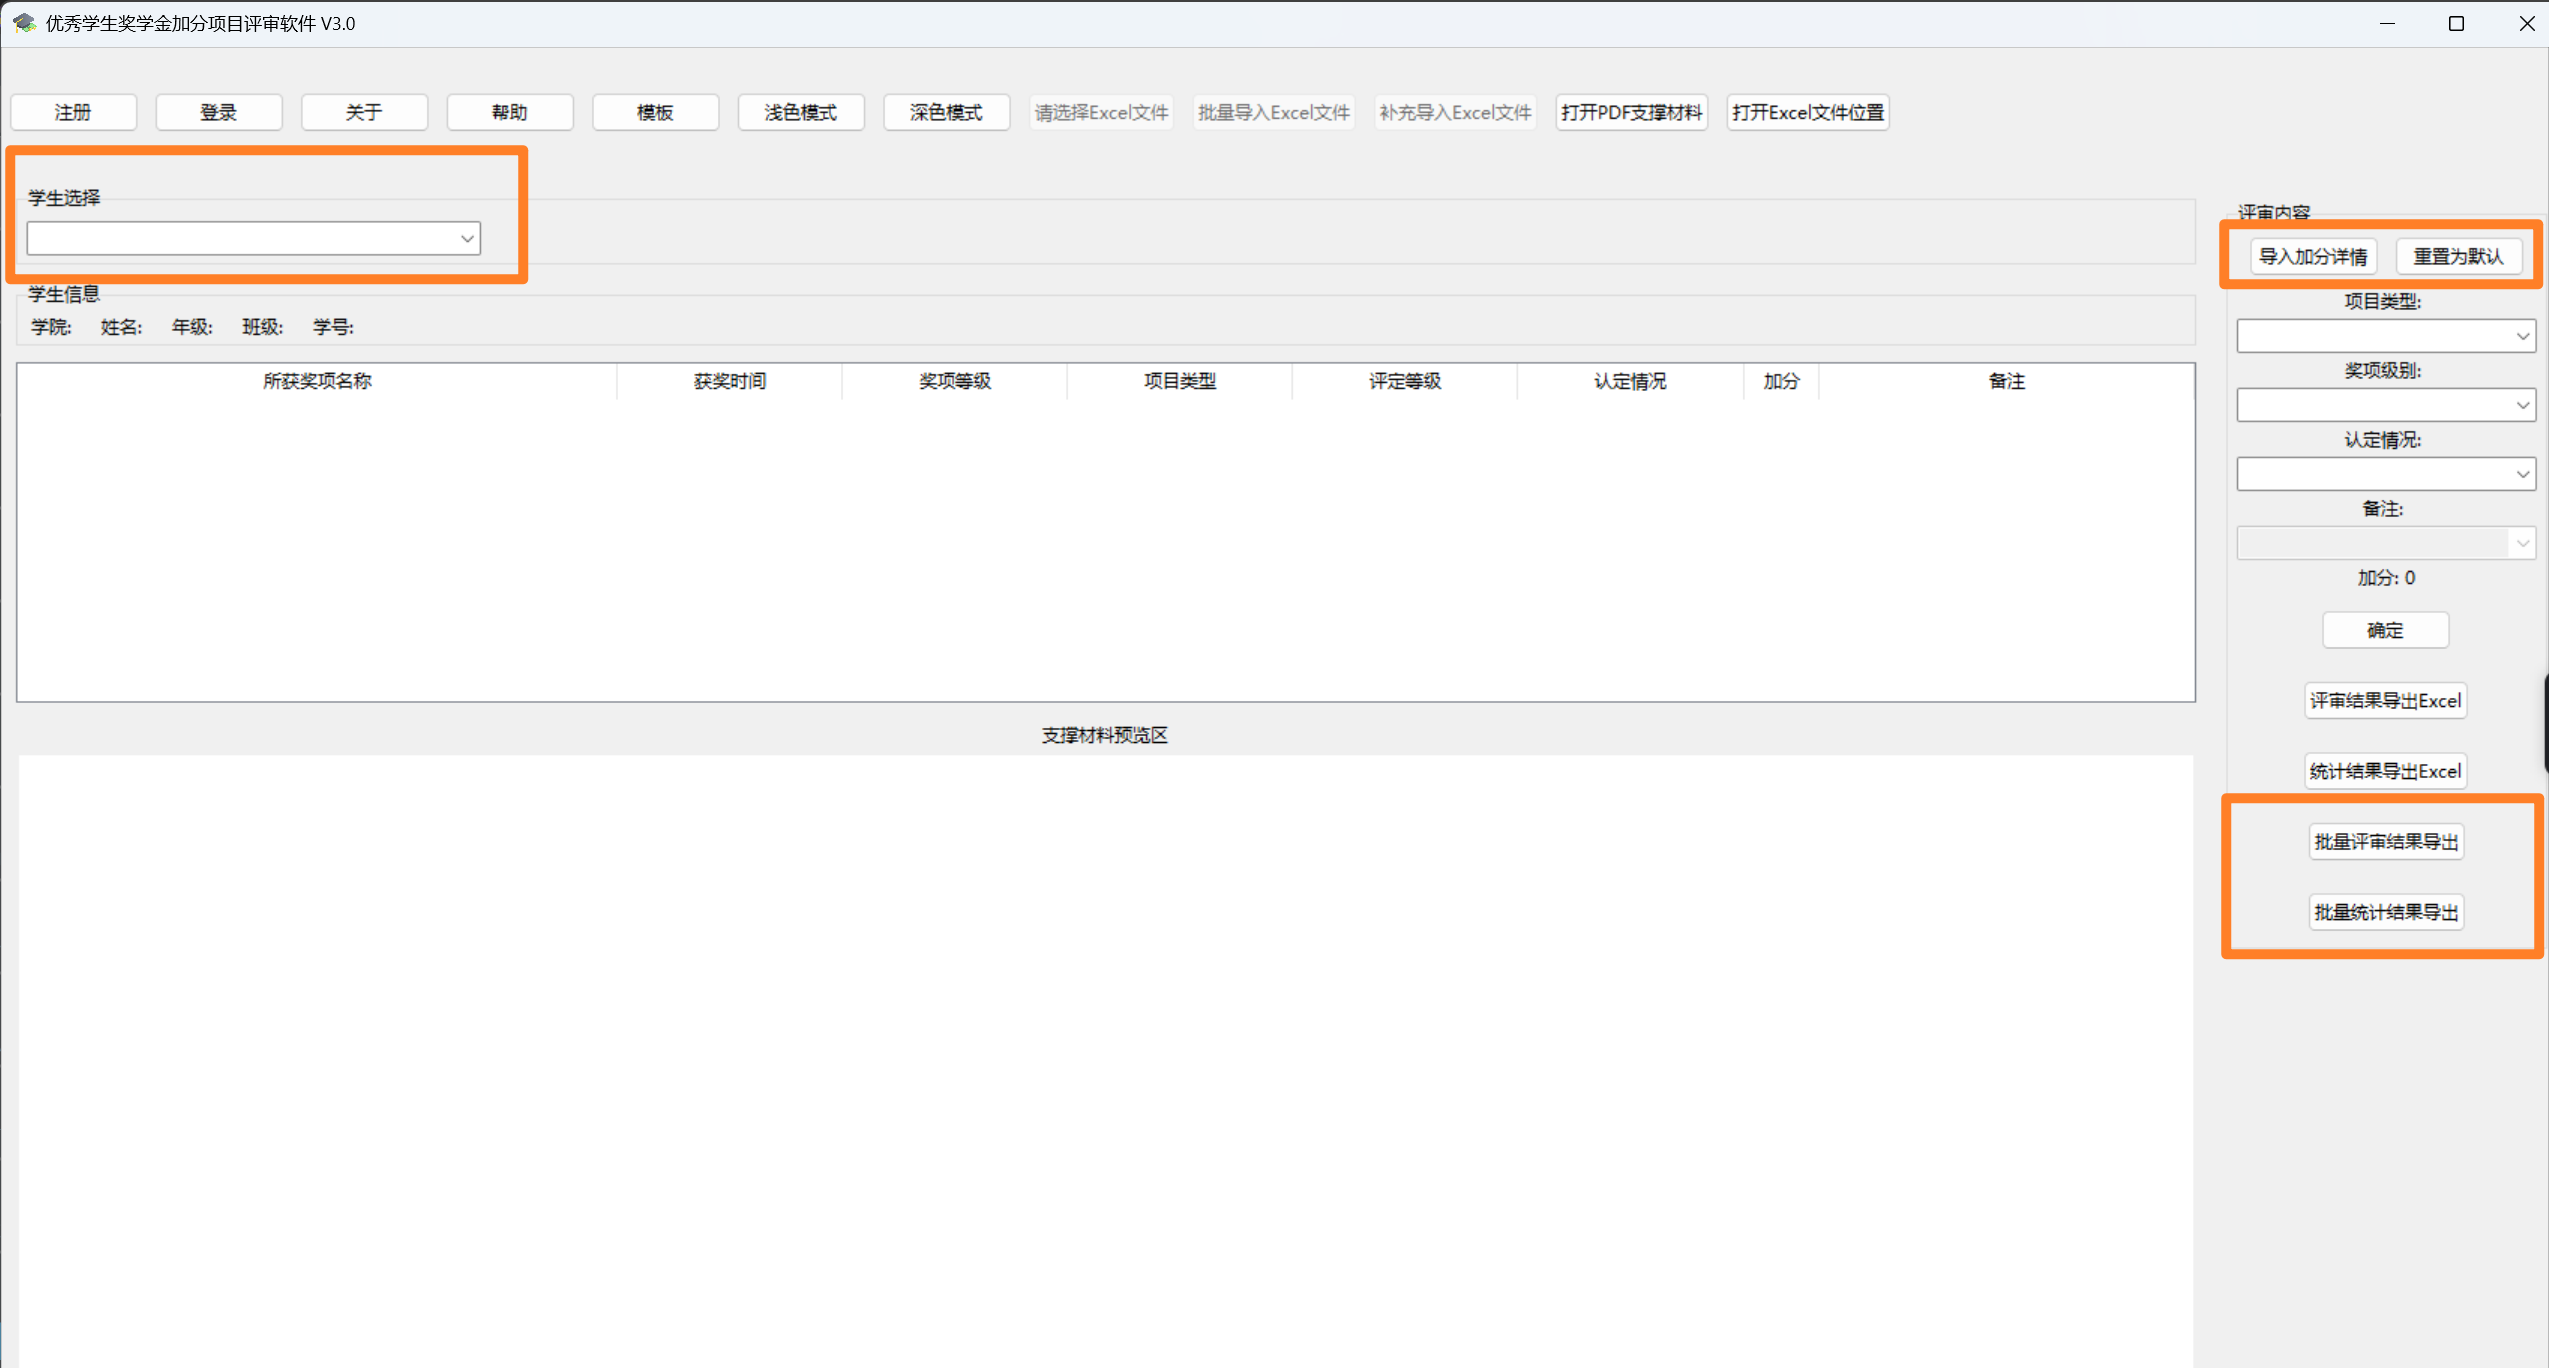
\includegraphics[width=0.7\linewidth]{fig/3.0评审界面新功能}
	\caption{版本V2.0评审界面新功能按钮展示}
	\label{fig:版本V3.0评审界面新功能按钮展示}
\end{figure}

{\color{myred}
	版本V3.0在评审界面新增了“历史记录”入口（仅在数据库功能启用且数据库可用时显示）。点击该入口将打开历史记录查询窗口，支持查询批次、学生、申请与评审记录，并支持导出查询结果或导出完整评审批次。
}

{\color{myred}
	版本V3.0在评审界面“确定”按钮下方新增了“撤销”和“重做”两个按钮，分别用于撤销和重做最近一次的评审操作。同时新增了“统计面板”按钮（用于打开数据可视化窗口）、“导出PDF报告”按钮（导出当前学生的A4格式PDF评审报告）和“批量PDF汇总”按钮（导出所有学生的PDF排名汇总表）。
	% 【需补充截图：V3.0评审界面全貌——展示撤销/重做按钮、统计面板按钮、PDF导出按钮的位置，命名为 fig/V3.0_review_panel.png】
}

   \subsection{支撑材料预览区}
	如图\ref{fig:支撑材料预览区}所示，为版本V2.0添加的支撑材料预览区，可以显示导入的EXCEL文件的同一目录下的与“所获奖项名称”相同的文件名的图片（jpg、jpeg和png格式），如果文件为pdf文件，则会提示点击“打开PDF支撑材料”按钮进行打开。
	\begin{figure}[H]
		\centering
		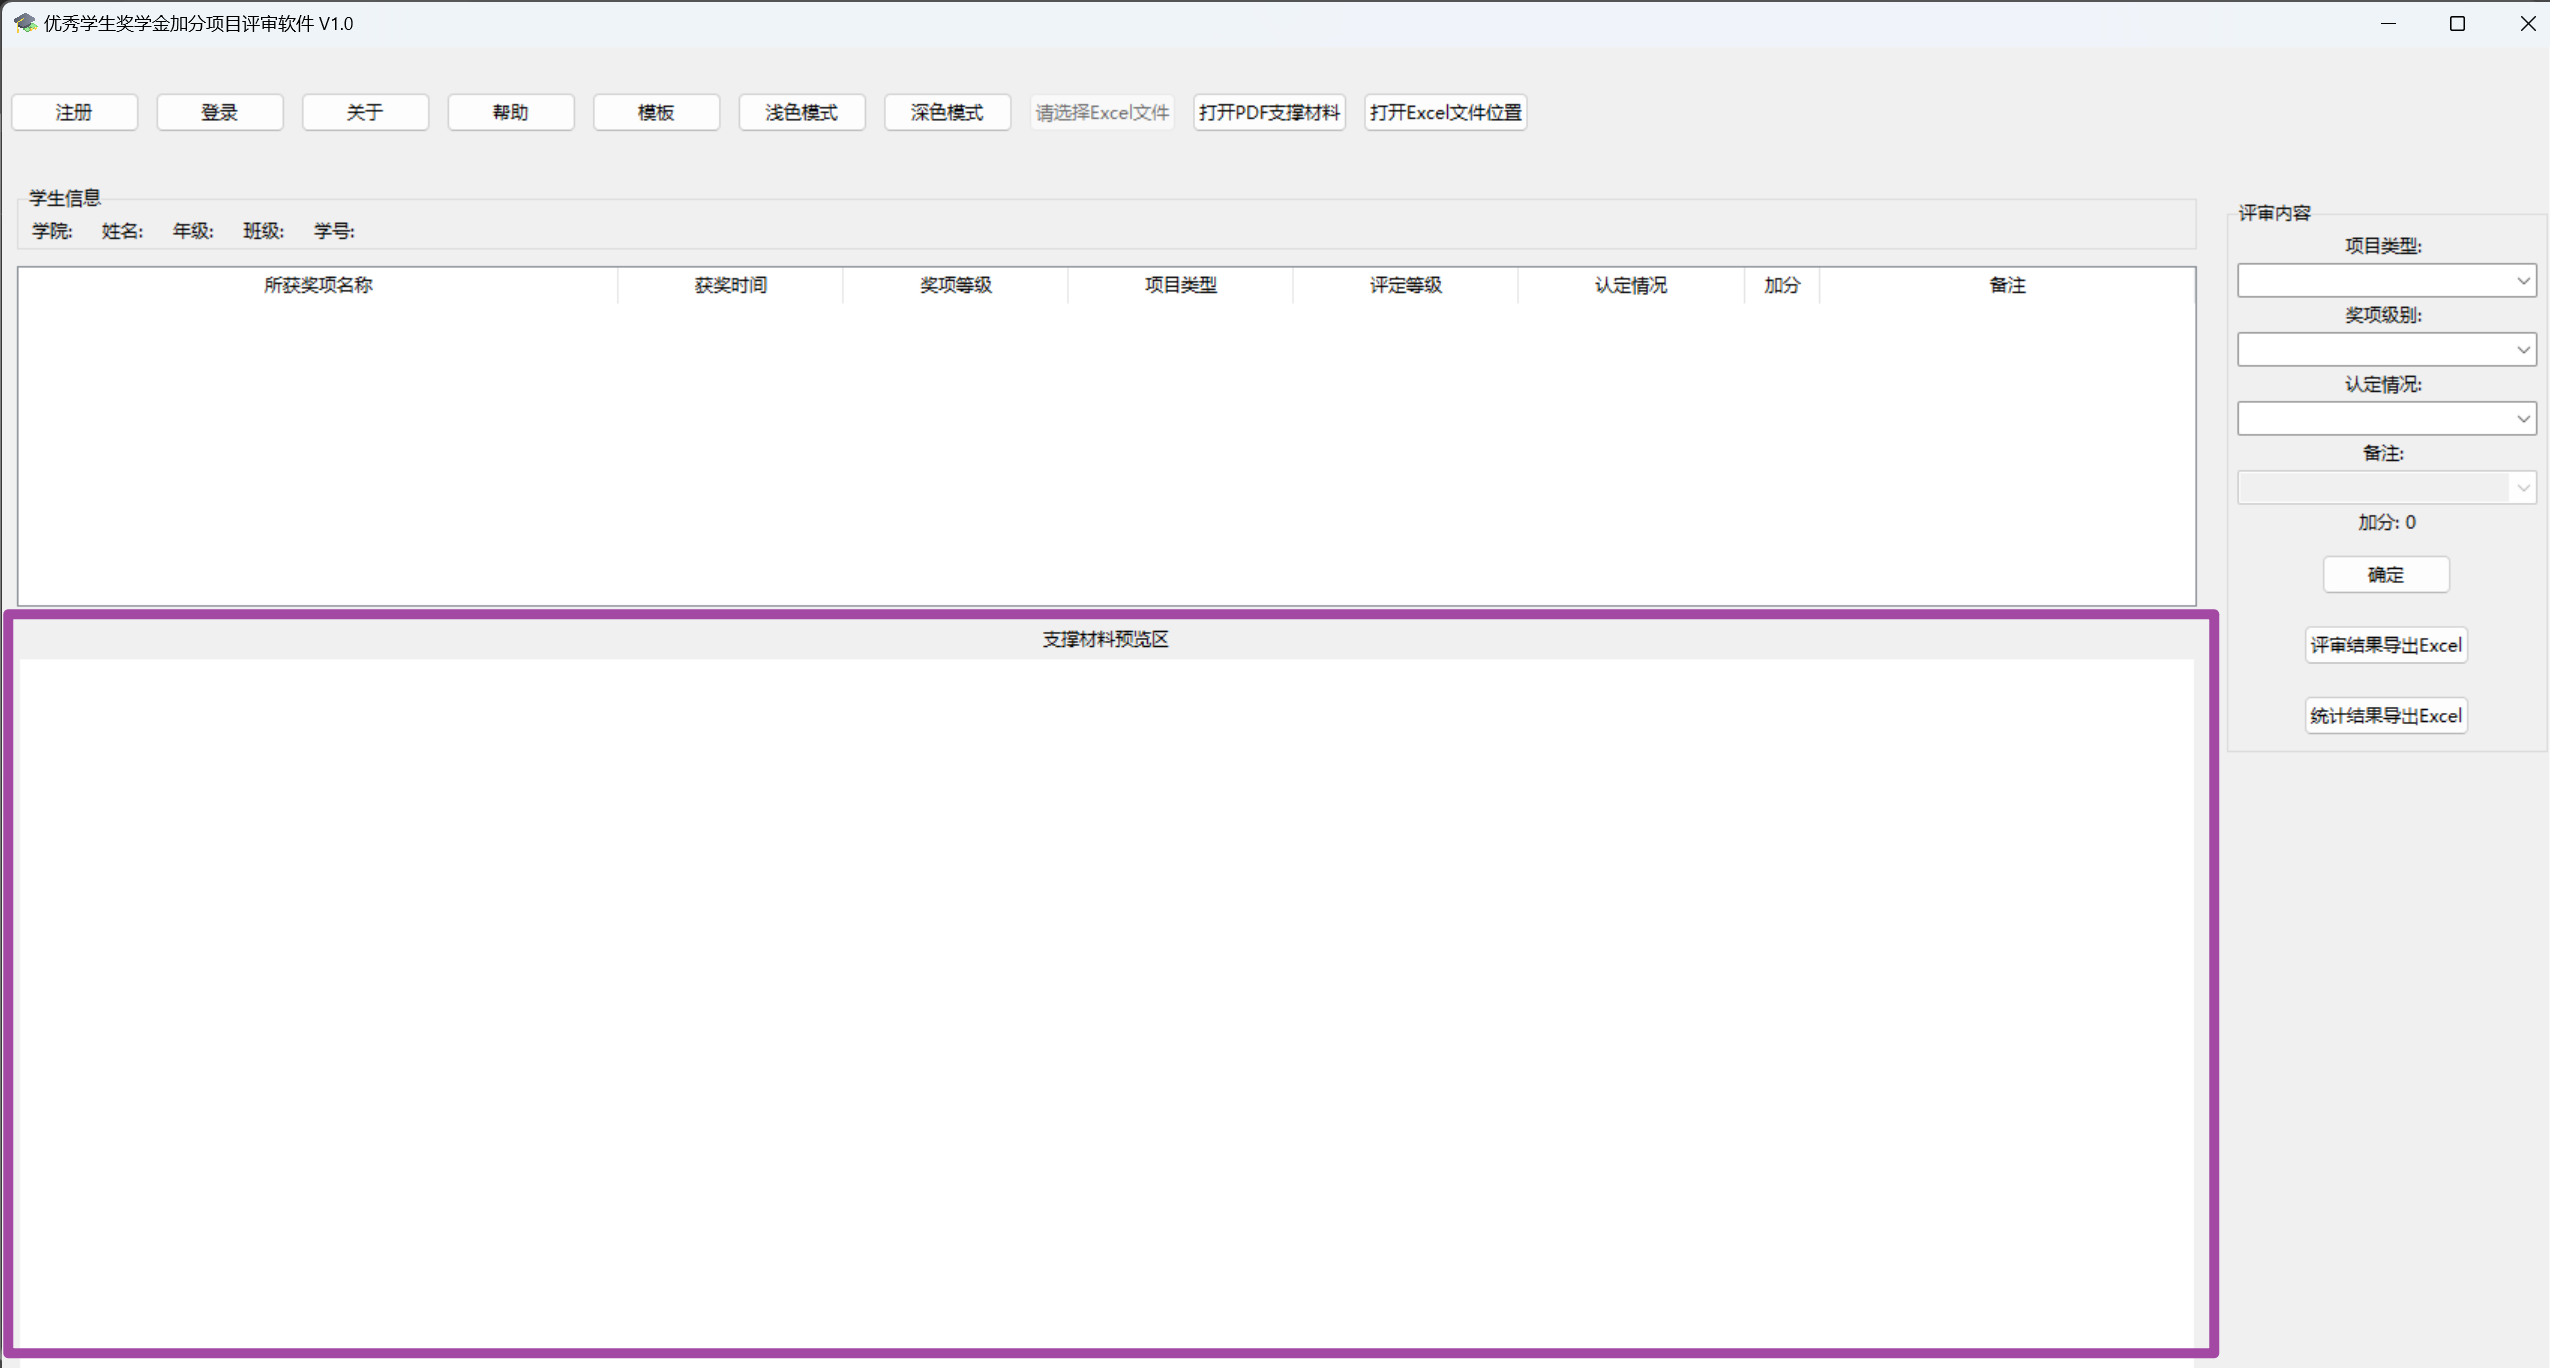
\includegraphics[width=0.7\linewidth]{fig/支撑材料预览区}
		\caption{支撑材料预览区}
		\label{fig:支撑材料预览区}
	\end{figure}

\newpage
